%%%%%%%%%%%%%%%%%%%%%%%%%%%%%%%%%%%%%%%%%%%%%%%%%%%%%%%%%%%%%%%%%%%%%%
% LaTeX Example: Project Report
%
% Source: http://www.howtotex.com
%
% Feel free to distribute this example, but please keep the referral
% to howtotex.com
% Date: March 2011 
% 
%%%%%%%%%%%%%%%%%%%%%%%%%%%%%%%%%%%%%%%%%%%%%%%%%%%%%%%%%%%%%%%%%%%%%%
% How to use writeLaTeX: 
%
% You edit the source code here on the left, and the preview on the
% right shows you the result within a few seconds.
%
% Bookmark this page and share the URL with your co-authors. They can
% edit at the same time!
%
% You can upload figures, bibliographies, custom classes and
% styles using the files menu.
%
% If you're new to LaTeX, the wikibook is a great place to start:
% http://en.wikibooks.org/wiki/LaTeX
%
%%%%%%%%%%%%%%%%%%%%%%%%%%%%%%%%%%%%%%%%%%%%%%%%%%%%%%%%%%%%%%%%%%%%%%
% Edit the title below to update the display in My Documents
%\title{Project Report}
%
%%% Preamble

%\documentclass[paper=a4, fontsize=11pt]{scrartcl}
%\usepackage[T1]{fontenc}
%\usepackage{fourier}
\documentclass [a4paper, 11pt, oneside, final]{article}
\usepackage[left=35mm,top=26mm,right=26mm,bottom=15mm]{geometry}
\usepackage{indentfirst}
\setlength{\parindent}{2em}
\setlength{\parskip}{1em}

\usepackage[english]{babel}															% English language/hyphenation
\usepackage[protrusion=true,expansion=true]{microtype}	
\usepackage{amsmath,amsfonts,amsthm} % Math packages
\usepackage[pdftex]{graphicx}	
\usepackage{url}
\graphicspath{{images/}}

%%% Custom sectioning
\usepackage{sectsty}
\allsectionsfont{\centering}



%%% Custom headers/footers (fancyhdr package)
\usepackage{fancyhdr}
\pagestyle{fancyplain}
\fancyhead{}											% No page header
\fancyfoot[L]{}											% Empty 
\fancyfoot[C]{}											% Empty
\fancyfoot[R]{\thepage}									% Pagenumbering
\renewcommand{\headrulewidth}{0pt}			% Remove header underlines
\renewcommand{\footrulewidth}{0pt}				% Remove footer underlines
\setlength{\headheight}{13.6pt}


%%% Equation and float numbering
\numberwithin{equation}{section}		% Equationnumbering: section.eq#
\numberwithin{figure}{section}			% Figurenumbering: section.fig#
\numberwithin{table}{section}				% Tablenumbering: section.tab#


%%% Maketitle metadata
\newcommand{\horrule}[1]{\rule{\linewidth}{#1}} 	% Horizontal rule

\title{
		%\vspace{-1in} 	
		\usefont{OT1}{bch}{b}{n}
		\normalfont \Large \textsc{Statistical Natural Language Processing}\\ \textsc{Brandeis University} \\ \textsc{Fall 2015}  \\[25pt]
		\horrule{0.5pt} \\[0.4cm]
		\huge Analysis of YouTube Spam\\
		\horrule{2pt} \\[0.5cm]
}

\author{
	\normalfont 								
	\normalsize
        Jing Zou\\Huilin Gang \\
	\normalsize        
	\today
}

\date{}


%%% Begin document
\begin{document}
\maketitle

\newpage

\section{Purpose}
YouTube becomes more lucrative targets for spammers hoping to attract unsuspecting users to malicious websites, where a variety of threats such as scams (phishing, e-commerce) and malware can be found. We demonstrate how such of these can be tracked over time using prime SVM and Neural Network Model. Based on both models, we will estimate how these models work with our dataset. 
\section{Dataset Collection}
Following the lead of earlier related YouTube research, a data set was collected in order to permit the investigation of contemporary spam comment activity.These data are retrieved from YouTube API which provides access to video and user information. Data retrieval ran from October 31st, 2011 to January 17th, 2012.\\

\begin{table}[h!]
  \begin{center}
    \caption{Data Properties}
    \label{tab:table1}
    \begin{tabular}{ccccccccc}
    \\
    \hline
      Videos & 6407\\
      \hline
     Total comments & 6431471 \\
      \hline
      Total users & 2860264  \\
       \hline  
     Spam comment users & 177542 \\
      \hline
    \end{tabular}
  \end{center}
\end{table}

\begin{table}[h!]
  \begin{center}
    \caption{Sample data from training dataset}
    \label{tab:table1}
    \begin{tabular}{ccccccccc}
    \\
    \hline
      published & videoId & userId & commentText & spam\\
      \hline
     1321991078000 & video1473 & user812400 & i lost count after last night at the gay bar & false \\
    \end{tabular}
  \end{center}
\end{table}

\section{Preprocessing}
Our methodology requires the generation of a network to represent the comment posting activity of users to a set of videos.  Initially, the focus of the evaluation is English-language spam comments. \\

The original dataset is way to large for us to train our model and go on with experiments. Therefore, we prepared the datasets with 100000 comments. This  dataset will be our original dataset\\

Also, to extract the English comments in the original dataset, we included the ENCHANT package in our preprocessing. We tried two different methods to extract the English comments. For the first one, we put the whole sentence for ENCHANT to check and collect those with only exact English words. This method works poor for the reason that it only extracts the simple comment with less words like "Good!". Also, most of the comments are same. Therefore, we tried the second method to check the percentage of English words in the sentence. Before we do the extraction, we included NLTK tokenization tool to tokenize the comment first.

\section{Methodologies}
We will implement both Support Vector Machine and Neural Network models in our final project to classify the spam comment. The optional model comes Network Motif Analysis, which is generated in the previous research of Youtube spam analysis [Derek O Callaghan, Martin Harrigan, Joe Carthy, P adraig Cunningham]. We will implemented it if we have enough time, otherwise we will just add it into our experimentation.
\begin{enumerate}
\item SVM \\
Our focus is how SVM can have good practical performance scaled to work with large training sets. We are going to implement algorithms use variant of primal stochastic gradient descent(SGD).
\begin{enumerate}
\item Generalization \\
A learning problem mush have a measure that says how good and algorithm performs on the task. A universal goal is $generalization$. We try to minimize some function over the training set like: $$\hat{g}(\theta) = \frac{1}{n}\sum_{i=1}^{n} L(x_{i}, y_{i}; \theta)$$ where L is a loss function.

\item Regularization \\
Regularization refers to augmenting the objective function g($\theta$) with an extra term that penalizes complex $\theta$ vectors. Therefore, the general form becomes $$\hat{g}(\theta) = \frac{1}{n}\sum_{i=1}^{n} L(x_{i}, y_{i}; \theta) + r(\theta)$$ where r($\theta$) is a regularization term.

\item Stochastic Gradient Descent \\
Gradient method computes $\theta$ = argmin $\hat{g}(\theta)$, where $\hat{g}(\theta)$ is the sum of empirical loss and regularization terms.
Stochastic Gradient Descent(SGD) is a simple yet very efficient approach to discriminative learning of linear classifiers under convex loss functions such as Support Vector Machines. It has been successfully applied to large-scale and sparse machine learning problems often encountered in text classification. We do not compute the gradient using the entire training set, however with respect to only a single randomly chosen example. The update rule is then:
$$ \theta_{t+1} = \theta_{t} - \eta_{t} \nabla  L(x_{i(t)}, y_{i(t)}; \theta_{t}) - \eta_{t} \nabla_{r}(\theta_{t})$$ where $i(t)$ is an index drawn randomly from \{1, 2, ..., n\}.
In expectation, this update is the same as gradient descent, because $E_{i(t)}[ l(x_{i(t)}, y_{i(t)}; \theta_{t})] =  \frac{1}{n}\sum_{i} l(x_{i}, y_{i}; \theta)$ \\

\item The primal SVM formulation\\
There are two ways of treating the SVM problem. The classical method is the hard margin SVM[Vapnik and Lerner, 1963], which assumes that the dataset is linearly separable: hence every point must be correctly classified by the maximum margin hyperplane. The soft margin SVM [Bennett and Mangasarian, 1992, Cortes and Vapnik, 1995] allows for some points to be misclassified, but penalizes these points appropriately. We implemented the latter represented with the following optimization problem.\\
In contrast to (batch) gradient descent, SGD approximates the true gradient of $E(w, b)$ by considering a single training example at a time.\\
By implementing a first-order SGD learning routine, the algorithm iterates over the training examples and for each example updates the model parameters according to the update rule given by $$\theta \leftarrow \theta - \eta(\alpha \frac{\partial r(\theta)}{\partial \theta} + \frac{\partial L(\theta^Tx_{i} + b, y_{i})}{\partial \theta})  $$ 
where $\eta$ is the learning rate which controls the step-size in the parameter space. The intercept $b$ is updated similarly but without regularization.\\
The learning rate $\eta$ can be either constant or gradually decaying. We give the default learning rate to be 
$$ \eta^{(t)} = \frac{1}{\alpha(t_{0} + t)}$$

\end{enumerate}

\item Neural Network  \\
Instead of using bag-of-word representation, we plan to use word-cluster representation. Brown clustering algorithm introduces a good way to do clustering. \\
\begin{enumerate}

\item Brown Clustering \\
Word embedding is very useful in deep learning area that mapped words to vectors in a low dimensional space, comparing to the vocabulary size. One of popular approaches such is Brown clustering algorithm. Brown clustering is an agglomerative clustering algorithm that clusters words based on which words precede or follow them. Each word is initially assigned to its own cluster. Then we will consider merging each pair of clusters. Two words are merged that have similar probabilities of preceding and following words. Clustering proceeds until all words are in one big cluster. This model has the same general form as a hidden Markov model. Given cluster membership indicators $c_i$ for the tokens $w_i$ in a text, the probability of the $w_i$ given $w_{i-1}$ is given by\\
$$P(w_i | w_{i-1}) = P(c_i|c_{i-1})P(w_i|c_i)$$
\item Neural Network Language Model\\
Neural neworks are typically organized in layers. Layers are made up of a number of interconnected 'nodes' which contain an 'activation function'. Patterns are presented to the network via the 'input layer', which communicates to one or more 'hidden layers' where the actual processing is done via a system of weighted 'connections'. The hidden layers then link to an 'output layer' where the answer is output as shown in the graphic below. 
For example, a neural network structure for 3 classes, 8 features and 2 feature groups per class:
\begin{figure}[h]
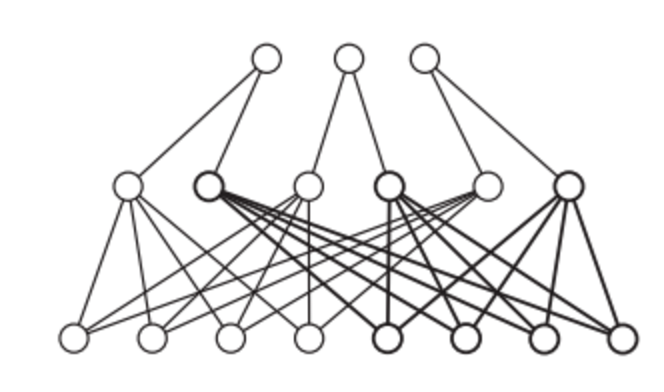
\includegraphics[width = 10cm]{nn}
\end{figure}			        


Let $n$ be the number of output units, $g$ the number of feature groups per class and $gn$ the number of hidden units given by the product.
The output of the network for an input $x$ is:
$$ f(x) = W_{o}tanh(W_{h}x + bh) + b_{o}$$ where $W_{o}$ is a $n \times gn$ matrix, $W_{h}$ is a $gn \times |V|$ matrix, $b_{o}$ is a vector of dimension
$n$ and $bn$ is a vector of dimension $gc$.\\
Let ${w_{1}, . . . , w_{n}}$ be a set of weight vectors derived from a linear model. Let ${\pi_{1}, . . . , \pi_{g}}$ be a random partition of the set of feature indices ${1, 2, . . . , |V |}$  into g equally-sized groups. For each class $c$, associate $g$ hidden units ${h_{1}^{(c)}, . . . , h_{g}^{(c)}}$.
 For all $i \in [1, g]$ and $j \in [1, |\pi(i) |]$, the weight of the connection between $h_{1}^{(c)}$ and the input unit $x_{\pi_{j}}^{(i)} $ is given by $(W_{c})_{\pi_{j}^{i}}$
\end{enumerate}
 
\end{enumerate}

\section{Experiments and Result}
\begin{enumerate}
\item Support Vector Machines \\
\begin{table}[h!]
  \begin{center}
    \caption{SVM accuracy with training data set 50000 and learning rate 0.0001}
    \label{tab:table1}
    \begin{tabular}{ccccccccc}
    \\
    \hline
     SGD PRIMAL SVM CLASSIFIER & 93.38\% \\
      \hline
     LINEAR SVM CLASSIFIER(SKLEARN) & 92.61\% \\
      \hline
     SGD CLASSIFIER(SKLEARN) & 93.32\%  \\
      \hline
    \end{tabular}
  \end{center}
\end{table}

Here is a figure with different training dataset associated with accuracy in the three model
\begin{figure}[h]
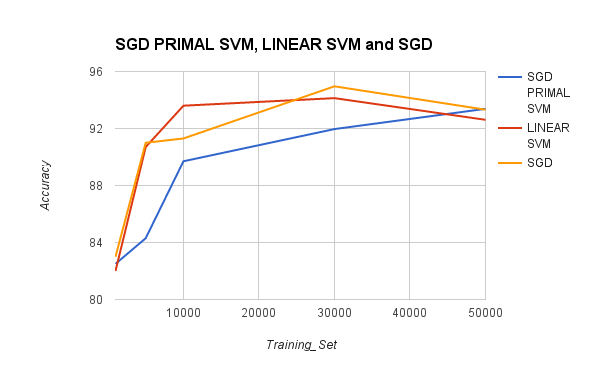
\includegraphics[width = 10cm]{svm}
\end{figure}
\item Neural Network \\
\end{enumerate}


\section{References}
\noindent O'Callaghan, Derek, et al. "Network Analysis of Recurring YouTube Spam Campaigns." ICWSM. 2012.\\
\noindent Menon, Aditya Krishna. "Large-scale support vector machines: algorithms and theory." Research Exam, University of California, San Diego (2009): 1-17.\\
\noindent Chapelle, Olivier. "Training a support vector machine in the primal." Neural Computation 19.5 (2007): 1155-1178.\\
%%% End document
\end{document}